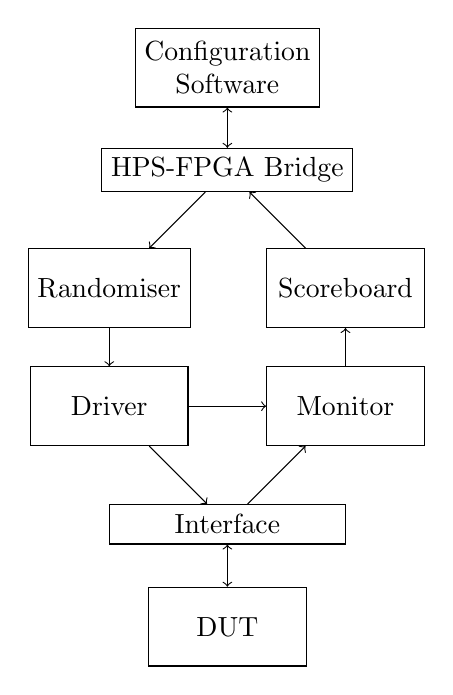
\begin{tikzpicture}
    \tikzset{block/.style= {draw,
                            rectangle,
                            align=center,
                            minimum width=2cm,
                            minimum height=1cm},
             inter/.style= {draw,
                            rectangle,
                            minimum width=3cm,
                            minimum height=0.5cm},
            }
    \path
    (0,3.5)    node[block](r) {Randomiser}
    (0,2)      node[block](d) {Driver}
    (1.5,0.5)  node[inter](i) {Interface}
    (1.5,-0.8) node[block](t) {DUT}
    (3,3.5)    node[block](s) {Scoreboard}
    (3,2)      node[block](m) {Monitor}
    (1.5,5)    node[inter](b) {HPS-FPGA Bridge}
    (1.5,6.3)  node[block](w) {Configuration\\Software}
    ;
    \draw[->]  (r) -- (d);
    \draw[->]  (d) -- (i);
    \draw[<->] (i) -- (t);
    \draw[->]  (i) -- (m);
    \draw[->]  (m) -- (s);
    \draw[->]  (b) -- (r);
    \draw[->]  (s) -- (b);
    \draw[<->] (b) -- (w);
    \draw[->]  (d) -- (m);
\end{tikzpicture}